\documentclass{standalone}
\usepackage[dvipsnames]{xcolor}
\usepackage{tikz}                       % Graphen und kommutative Diagramme
\usetikzlibrary{patterns}               % Um schraffierte Formen in der tikzpicture-Umgebung zu zeichnen.
\newcommand{\ul}[1]{\underline{\smash{#1}}}

\begin{document}

\centering
\begin{minipage}{.4\textwidth}
\centering
\resizebox{!}{4.5cm}{
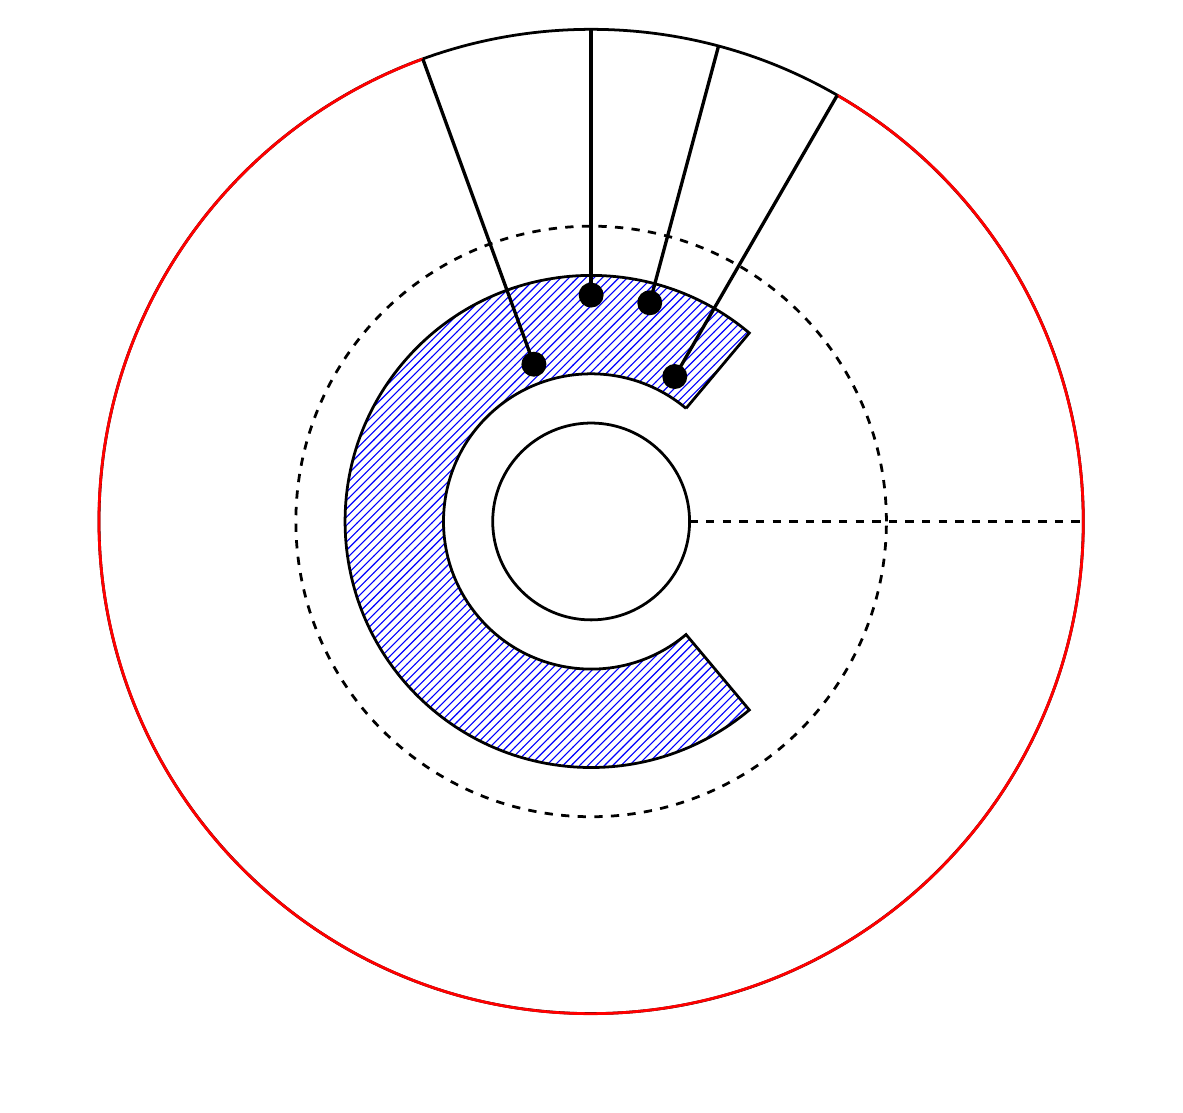
\begin{tikzpicture}[x=1.25cm, y=1.25cm, line width=1pt]
    % draw inner and outer circles
    \draw[color=black] (0, 0) circle (1);
    \draw[color=black] (0, 0) circle (5);
    \draw[color=black, dashed] (0, 0) circle (3);
    \draw[color=red] (60 : 5) arc [radius = 5, start angle = 60, delta angle = -310];

    % draw 0 line
    \draw[color=black, dashed] (0 : 1) -- (0 : 5); 
   
    % draw shaded slit box
    \filldraw[pattern=north east lines, pattern color=blue] 
      (50 : 1.5) -- (50 : 2.5) arc [radius = 2.5, start angle = 50, delta angle = 260] 
	       -- (310 : 1.5) arc [radius = 1.5, start angle = 310, delta angle = -260] ;
    
    % draw slits
    \draw[color=black, line width=1.2pt] (60 : 5) -- (60 : 1.7);
    \filldraw[color = black, fill = black] (60 : 1.7) circle (4pt);

    \draw[color=black, line width=1.2pt] (90 : 5) -- (90 : 2.3);
    \filldraw[color = black, fill = black] (90 : 2.3) circle (4pt);
     
    \draw[color=black, line width=1.2pt] (110 : 5) -- (110 : 1.7);
    \filldraw[color = black, fill = black] (110 : 1.7) circle (4pt);
     
    \draw[color=black, line width=1.2pt] (75 : 5) -- (75 : 2.3);
    \filldraw[color = black, fill = black] (75 : 2.3) circle (4pt);

\end{tikzpicture}
}
\end{minipage}

\centering
\begin{minipage}{.4\textwidth}
\centering
\resizebox{!}{4.5cm}{
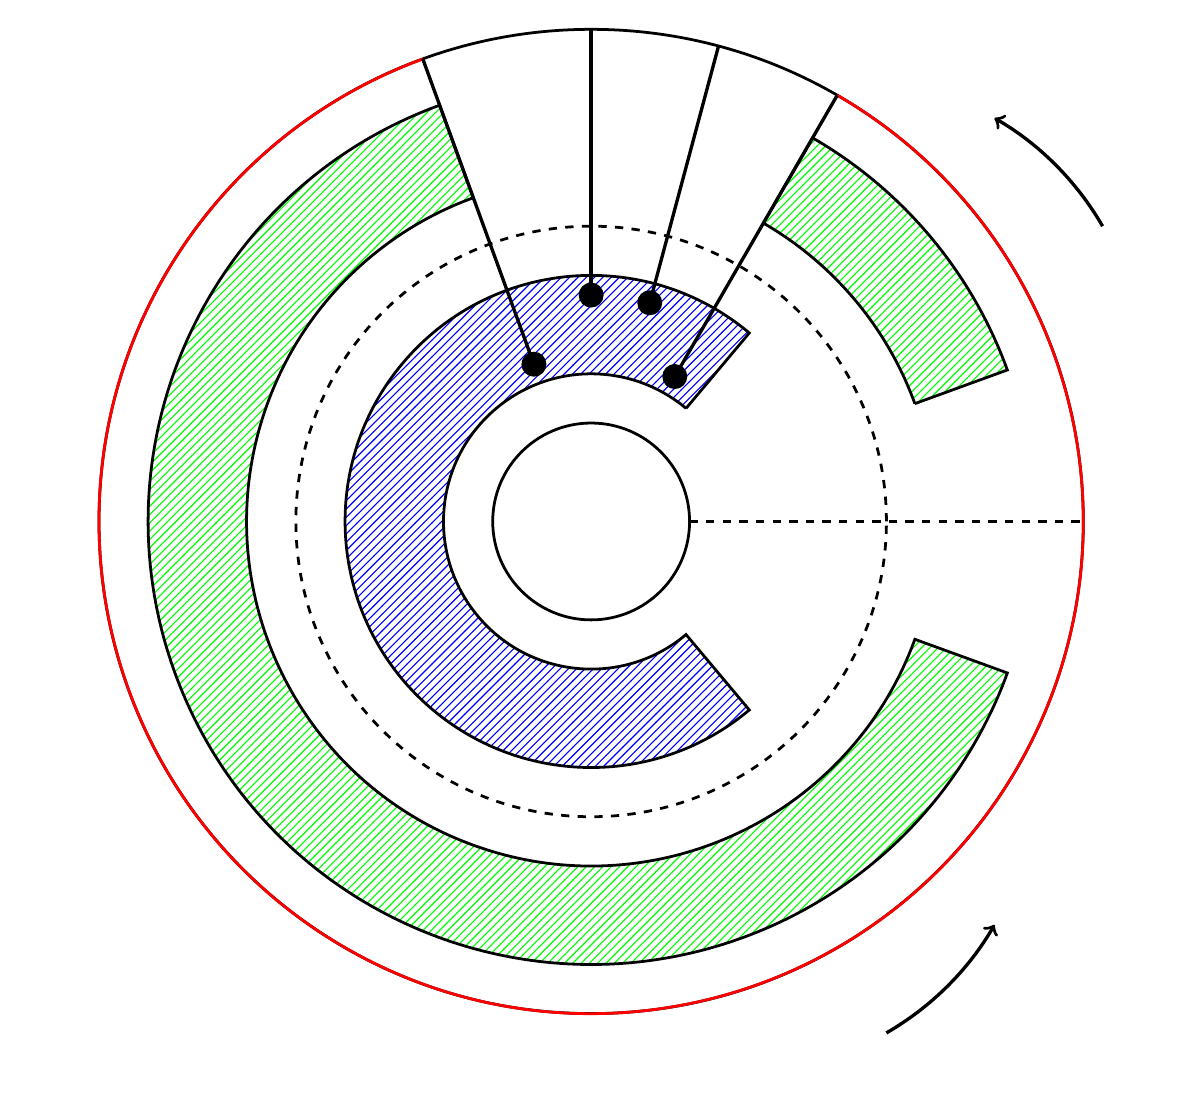
\begin{tikzpicture}[x=1.25cm, y=1.25cm, line width=1pt]
    % draw inner and outer circles
    \draw[color=black] (0, 0) circle (1);
    \draw[color=black] (0, 0) circle (5);
    \draw[color=black, dashed] (0, 0) circle (3);
    \draw[color=red] (60 : 5) arc [radius = 5, start angle = 60, delta angle = -310];

    % draw 0 line
    \draw[color=black, dashed] (0 : 1) -- (0 : 5); 
    
    % draw shaded slit box
    \filldraw[pattern=north east lines, pattern color=blue] 
      (50 : 1.5) -- (50 : 2.5) arc [radius = 2.5, start angle = 50, delta angle = 260] 
	       -- (310 : 1.5) arc [radius = 1.5, start angle = 310, delta angle = -260] ; 
    
    \filldraw[pattern=north east lines, pattern color=green] 
      (110 : 3.5) -- (110 : 4.5) arc [radius = 4.5, start angle = 110, delta angle = 230] 
	       -- (340 : 3.5) arc [radius = 3.5, start angle = 340, delta angle = -230];
    \filldraw[pattern=north east lines, pattern color=green] 
      (20 : 3.5) -- (20 : 4.5) arc [radius = 4.5, start angle = 20, delta angle = 40] 
	       -- (60 : 3.5) arc [radius = 3.5, start angle = 60, delta angle = -40];
	       
     % draw slits
    \draw[color=black, line width=1.2pt] (60 : 5) -- (60 : 1.7);
    \filldraw[color = black, fill = black] (60 : 1.7) circle (4pt);

    \draw[color=black, line width=1.2pt] (90 : 5) -- (90 : 2.3);
    \filldraw[color = black, fill = black] (90 : 2.3) circle (4pt);
     
    \draw[color=black, line width=1.2pt] (110 : 5) -- (110 : 1.7);
    \filldraw[color = black, fill = black] (110 : 1.7) circle (4pt);
     
    \draw[color=black, line width=1.2pt] (75 : 5) -- (75 : 2.3);
    \filldraw[color = black, fill = black] (75 : 2.3) circle (4pt);
 
     % draw arrow
     \draw[->, line width = 1.2pt] (30 : 6) arc [radius = 3, start angle = 30, delta angle = 30];
     \draw[->, line width = 1.2pt] (300 : 6) arc [radius = 3, start angle = 300, delta angle = 30];
     
\end{tikzpicture}
}
\end{minipage}


\end{document}
